\documentclass[a4paper,11pt]{jsarticle}

% パッケージ
\usepackage[dvipdfmx]{hyperref}
\usepackage{pxjahyper}
\usepackage[dvipdfmx]{graphicx}
\usepackage{ascmac}
\usepackage{fancybox}
\usepackage{listings}
\usepackage{plistings}
\usepackage{color}
\usepackage{here}
\usepackage{amsmath,amsfonts}
\usepackage[utf8]{inputenc}
\usepackage{bm}
\usepackage{siunitx}
\usepackage{url}
% ページの周りの余白
\usepackage[top=10truemm,bottom=10truemm,left=25truemm,right=25truemm]{geometry}
% ページ番号の削除
\pagestyle{empty}

% URLの設定
\Urlmuskip=0mu  plus 10mu

% 色の定義
\definecolor{OliveGreen}{rgb}{0.0,0.6,0.0}
\definecolor{Magenta}{cmyk}{0, 1, 0, 0}
\definecolor{colFunc}{rgb}{1,0.07,0.54}
\definecolor{CadetBlue}{cmyk}{0.62,0.57,0.23,0}
\definecolor{Brown}{cmyk}{0,0.81,1,0.60}
\definecolor{colID}{rgb}{0.63,0.44,0}


\lstset{
  basicstyle={\ttfamily},
  identifierstyle={\small},
  commentstyle={\smallitshape},
  keywordstyle={\small\bfseries},
  ndkeywordstyle={\small},
  stringstyle={\small\ttfamily},
  frame={tb},
  breaklines=true,
  columns=[l]{fullflexible},
  numbers=left,
  xrightmargin=0zw,
  xleftmargin=3zw,
  numberstyle={\scriptsize},
  stepnumber=1,
  numbersep=1zw,
  lineskip=-0.5ex
}

\renewcommand{\lstlistingname}{Code}

% リンクの設定
\hypersetup{
  setpagesize=false,
  bookmarksnumbered=true,
  bookmarksopen=true,
  colorlinks=true,
  linkcolor=blue,
  citecolor=red,
}

\begin{document}

\section{実験1}
以下にソースコードとその実行結果を示す.
\begin{lstlisting}
  clear();
  s = %s;
  P = syslin('c', 3/(2*s+1));
  t = 0:0.1:20;
  u = ones(t);
  y = csim(u,t,P);
  xmin = 0; xmax = 20; ymin = -0.5; ymax = 3.5;
  scf(0);
  
  plot2d(t,u,style=color(0,0,255),rect=[xmin ymin xmax ymax]);
  
  plot2d(t,y,style=color(255,0,0),rect=[xmin ymin xmax ymax]);
  
  xtitle('Step Response', 'time[s]', 'u, y')
  xgrid();
  
  xs2png(0, 'experiment1-1.png')  
\end{lstlisting}
\begin{figure}[H]
  \centering
  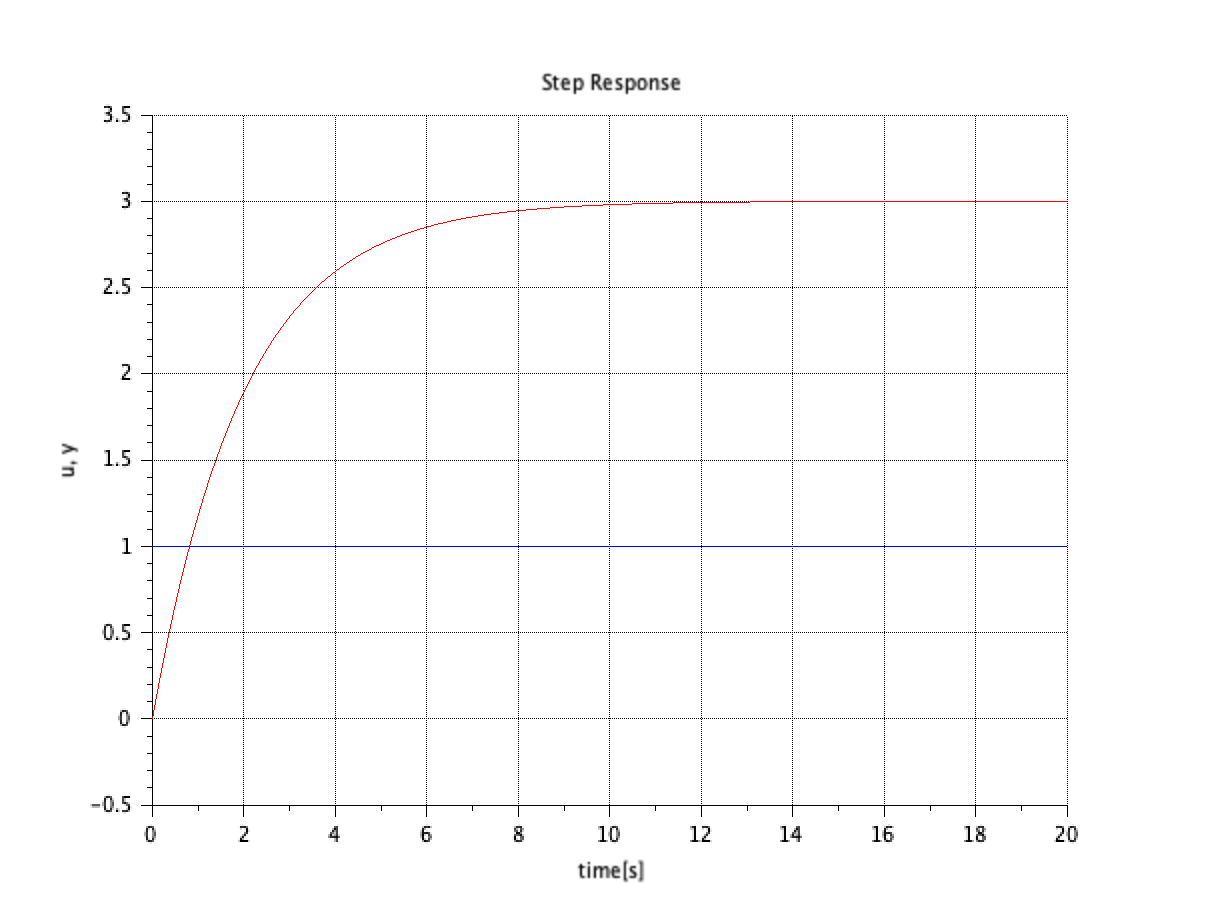
\includegraphics[width=0.8\linewidth]{picture/experiment1-1.png}
  \caption{実験1の実行結果}
  \label{1}
\end{figure}



\end{document}